%%%% Proceedings format for most of ACM conferences (with the exceptions listed below) and all ICPS volumes.
\documentclass[sigconf]{acmart}

\usepackage{caption}
\usepackage{subcaption}

\graphicspath{ {./images/} }

%%%% As of March 2017, [siggraph] is no longer used. Please use sigconf (above) for SIGGRAPH conferences.

%%%% Proceedings format for SIGPLAN conferences 
% \documentclass[sigplan, anonymous, review]{acmart}

%%%% Proceedings format for SIGCHI conferences
% \documentclass[sigchi, review]{acmart}

%%%% To use the SIGCHI extended abstract template, please visit
% https://www.overleaf.com/read/zzzfqvkmrfzn

%
% defining the \BibTeX command - from Oren Patashnik's original BibTeX documentation.
\def\BibTeX{{\rm B\kern-.05em{\sc i\kern-.025em b}\kern-.08emT\kern-.1667em\lower.7ex\hbox{E}\kern-.125emX}}
    
% Rights management information. 
% This information is sent to you when you complete the rights form.
% These commands have SAMPLE values in them; it is your responsibility as an author to replace
% the commands and values with those provided to you when you complete the rights form.
%
% These commands are for a PROCEEDINGS abstract or paper.
\copyrightyear{2018}
\acmYear{2018}
\setcopyright{acmlicensed}
\acmConference[Woodstock '18]{Woodstock '18: ACM Symposium on Neural Gaze Detection}{June 03--05, 2018}{Woodstock, NY}
\acmBooktitle{Woodstock '18: ACM Symposium on Neural Gaze Detection, June 03--05, 2018, Woodstock, NY}
\acmPrice{15.00}
\acmDOI{10.1145/1122445.1122456}
\acmISBN{978-1-4503-9999-9/18/06}

%
% These commands are for a JOURNAL article.
%\setcopyright{acmcopyright}
%\acmJournal{TOG}
%\acmYear{2018}\acmVolume{37}\acmNumber{4}\acmArticle{111}\acmMonth{8}
%\acmDOI{10.1145/1122445.1122456}

%
% Submission ID. 
% Use this when submitting an article to a sponsored event. You'll receive a unique submission ID from the organizers
% of the event, and this ID should be used as the parameter to this command.
%\acmSubmissionID{123-A56-BU3}

%
% The majority of ACM publications use numbered citations and references. If you are preparing content for an event
% sponsored by ACM SIGGRAPH, you must use the "author year" style of citations and references. Uncommenting
% the next command will enable that style.
%\citestyle{acmauthoryear}

%
% end of the preamble, start of the body of the document source.
\begin{document}

%
% The "title" command has an optional parameter, allowing the author to define a "short title" to be used in page headers.
% \title{The Name of the Title is Hope}
\title{POS Blockchain with Dynamically Changing Validators}

%
% The "author" command and its associated commands are used to define the authors and their affiliations.
% Of note is the shared affiliation of the first two authors, and the "authornote" and "authornotemark" commands
% used to denote shared contribution to the research.
\author{Ben Trovato}
\authornote{Both authors contributed equally to this research.}
\email{trovato@corporation.com}
\orcid{1234-5678-9012}
\author{G.K.M. Tobin}
\authornotemark[1]
\email{webmaster@marysville-ohio.com}
\affiliation{%
  \institution{Institute for Clarity in Documentation}
  \streetaddress{P.O. Box 1212}
  \city{Dublin}
  \state{Ohio}
  \postcode{43017-6221}
}

\author{Lars Th{\o}rv{\"a}ld}
\affiliation{%
  \institution{The Th{\o}rv{\"a}ld Group}
  \streetaddress{1 Th{\o}rv{\"a}ld Circle}
  \city{Hekla}
  \country{Iceland}}
\email{larst@affiliation.org}

\author{Valerie B\'eranger}
\affiliation{%
  \institution{Inria Paris-Rocquencourt}
  \city{Rocquencourt}
  \country{France}
}

\author{Aparna Patel}
\affiliation{%
 \institution{Rajiv Gandhi University}
 \streetaddress{Rono-Hills}
 \city{Doimukh}
 \state{Arunachal Pradesh}
 \country{India}}
 
\author{Huifen Chan}
\affiliation{%
  \institution{Tsinghua University}
  \streetaddress{30 Shuangqing Rd}
  \city{Haidian Qu}
  \state{Beijing Shi}
  \country{China}}

\author{Charles Palmer}
\affiliation{%
  \institution{Palmer Research Laboratories}
  \streetaddress{8600 Datapoint Drive}
  \city{San Antonio}
  \state{Texas}
  \postcode{78229}}
\email{cpalmer@prl.com}

\author{John Smith}
\affiliation{\institution{The Th{\o}rv{\"a}ld Group}}
\email{jsmith@affiliation.org}

\author{Julius P. Kumquat}
\affiliation{\institution{The Kumquat Consortium}}
\email{jpkumquat@consortium.net}

%
% By default, the full list of authors will be used in the page headers. Often, this list is too long, and will overlap
% other information printed in the page headers. This command allows the author to define a more concise list
% of authors' names for this purpose.
\renewcommand{\shortauthors}{Trovato and Tobin, et al.}

%
% The abstract is a short summary of the work to be presented in the article.
% \begin{abstract}
% A clear and well-documented \LaTeX\ document is presented as an article formatted for publication by ACM in 
% a conference proceedings or journal publication. Based on the ``acmart'' document class, this article presents
% and explains many of the common variations, as well as many of the formatting elements
% an author may use in the preparation of the documentation of their work.
% \end{abstract}

\begin{abstract}
    This paper proposes a new Proof of Stake type of cryptocurrency which uses a small subset of dynamically changing validators. The blockchain system takes into account the economics of currency exchanges so that the cryptocurrency can work as a unified currency. The system is democratic in that all the validators have equal votes. 
\end{abstract}

%
% The code below is generated by the tool at http://dl.acm.org/ccs.cfm.
% Please copy and paste the code instead of the example below.
%
\begin{CCSXML}
<ccs2012>
 <concept>
  <concept_id>10010520.10010553.10010562</concept_id>
  <concept_desc>Computer systems organization~Embedded systems</concept_desc>
  <concept_significance>500</concept_significance>
 </concept>
 <concept>
  <concept_id>10010520.10010575.10010755</concept_id>
  <concept_desc>Computer systems organization~Redundancy</concept_desc>
  <concept_significance>300</concept_significance>
 </concept>
 <concept>
  <concept_id>10010520.10010553.10010554</concept_id>
  <concept_desc>Computer systems organization~Robotics</concept_desc>
  <concept_significance>100</concept_significance>
 </concept>
 <concept>
  <concept_id>10003033.10003083.10003095</concept_id>
  <concept_desc>Networks~Network reliability</concept_desc>
  <concept_significance>100</concept_significance>
 </concept>
</ccs2012>
\end{CCSXML}

\ccsdesc[500]{Computer systems organization~Embedded systems}
\ccsdesc[300]{Computer systems organization~Redundancy}
\ccsdesc{Computer systems organization~Robotics}
\ccsdesc[100]{Networks~Network reliability}

%
% Keywords. The author(s) should pick words that accurately describe the work being
% presented. Separate the keywords with commas.
\keywords{datasets, neural networks, gaze detection, text tagging}

%
% A "teaser" image appears between the author and affiliation information and the body 
% of the document, and typically spans the page. 
\begin{teaserfigure}
  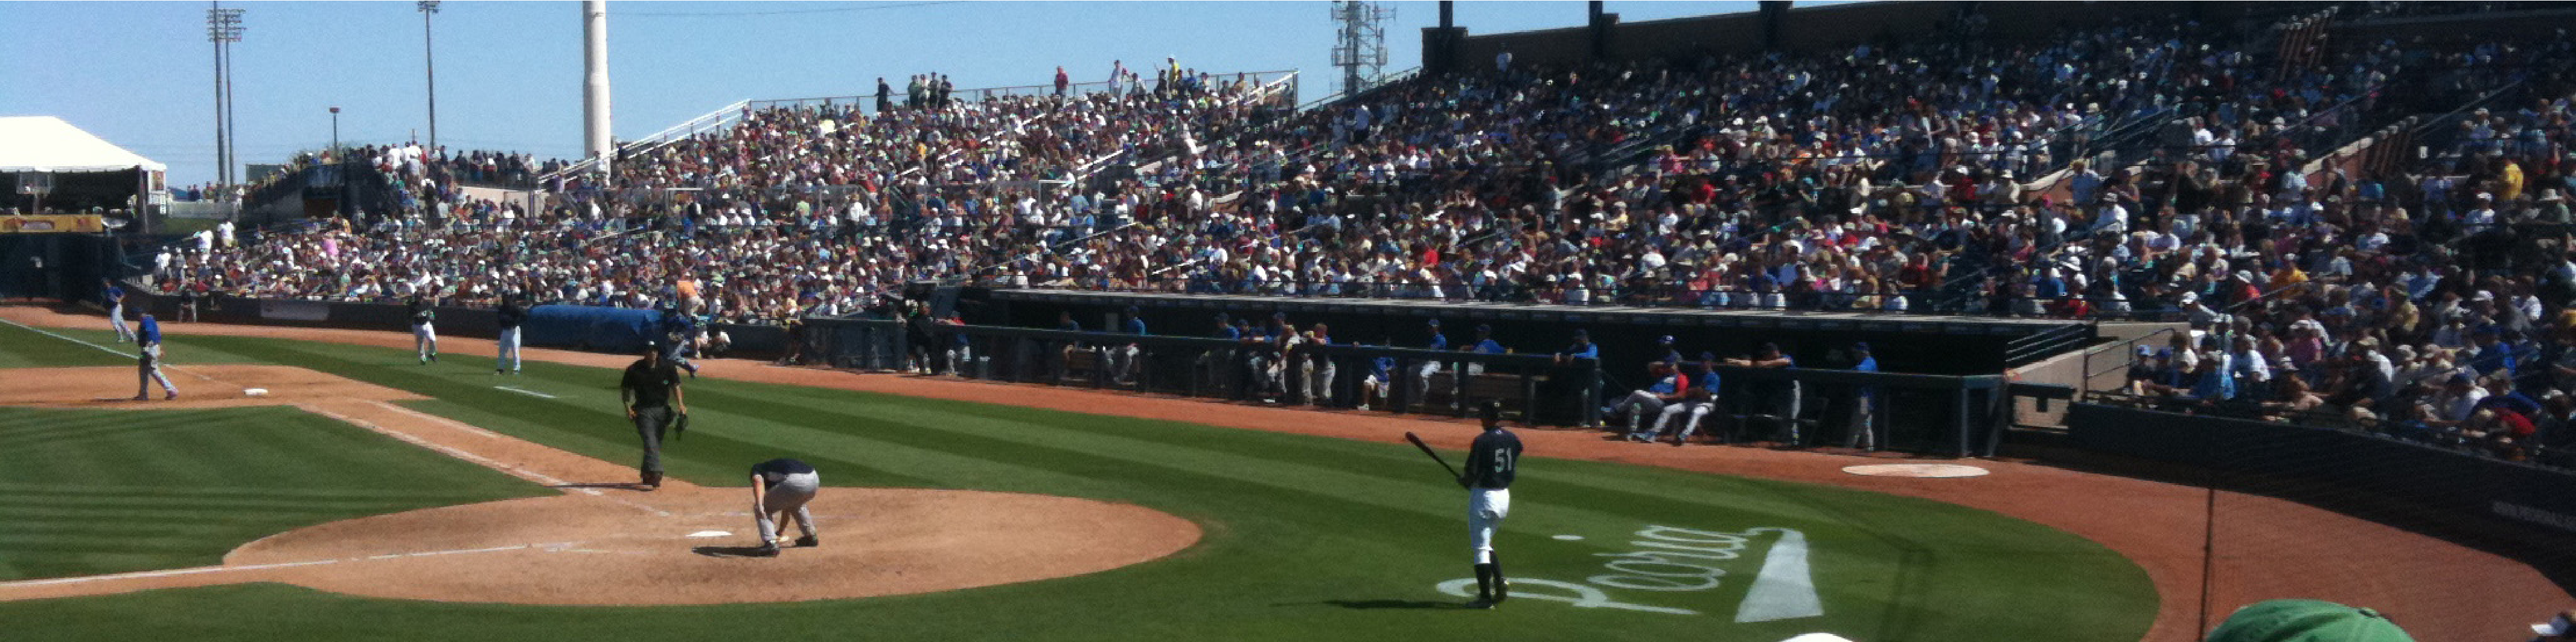
\includegraphics[width=\textwidth]{sampleteaser}
  \caption{Seattle Mariners at Spring Training, 2010.}
  \Description{Enjoying the baseball game from the third-base seats. Ichiro Suzuki preparing to bat.}
  \label{fig:teaser}
\end{teaserfigure}

%
% This command processes the author and affiliation and title information and builds
% the first part of the formatted document.
\maketitle

\section{Introduction}
%In 2008, the first ever cryptocurrency Bitcoin, solved the problem of double spending by using 

\subsection{What is a blockchain?}

A blockchain is a growing list of records, called blocks, which are linked using cryptography. Each block contains a cryptographic hash of the previous block, a timestamp, and transaction data (generally represented as a merkle tree root hash).

By design, a blockchain is resistant to modification of the data. It is "an open, distributed ledger that can record transactions between two parties efficiently and in a verifiable and permanent way". For use as a distributed ledger, a blockchain is typically managed by a peer-to-peer network collectively adhering to a protocol for inter-node communication and validating new blocks. Once recorded, the data in any given block cannot be altered retroactively without alteration of all subsequent blocks, which requires consensus of the network majority. Although blockchain records are not unalterable, blockchains may be considered secure by design and exemplify a distributed computing system with high Byzantine fault tolerance. Decentralized consensus has therefore been claimed with a blockchain.

\subsection{Problem Statement}

A blockchain system's throughput depends on the number of nodes participating in the validation of a transaction. More the number of nodes means more resistance to faults but resulting in higher latency and lower throughputs. The objective of this project is to propose a blockchain system where the number of validators is determined by the market dynamics.


\section{Motivation}

\subsection{State Machine Replication}

In computer science, state machine replication or state machine approach is a general method for implementing a fault-tolerant service by replicating servers and coordinating client interactions with server replicas.


Blockchain systems are an example of such a system where a ledger of committed transactions acts as a common state between the replicas. These replicas are also known as miners. In a blockchain system, a leader is chosen to commit the new block to the ledger, and the commit is successful only when a consensus is reached on it. This consensus can be reached via two methods, Proof of Work based consensus or Proof of Stake based consensus.

% \section{Types of faults}

% \subsection{Crash Faults}

% A replica is said to be crash-faulty if it stops all computation and communication.

% \subsection{Byzantine Faults}

% A replica is said to be Byzantine or non-crash faulty if it acts arbitrarily, but cannot break cryptographic primitives we use (crypto- graphic hashes, MACs, message digests and digital signatures).

% \subsection{Network Faults}

% A network fault is defined as the inability of some correct replicas to communicate with each other in a timely manner, that is, when a message exchanged between two correct replicas cannot be delivered and processed within delay $\Delta$, known to all replicas.

\subsection{Proof Of Work based consensus}

In Proof of Work based consensus, the miners compete against each other to complete transactions on the network and get rewarded. The miners are required to solve a hard problem (Eg : Finding a number which when concatenated with the current block of transactions produces a hash which is less than a given number). Whichever miner solves the problem first becomes the leader for the current round and the number acts as his proof of work. The miner then gets to commit the next block to the ledger. To take over the system, an adversary needs to own more than half of the computation power in the network. This consensus system though secured has certain drawbacks. 
\begin{enumerate}
  \item To make sure that all the miners are updated with the current ledger and to generate the consensus for the next block, it is important for the system to have a minimum amount of delay between commitment of two consecutive blocks. And, as the number of miners grow, this delay increases and hence the latency increases too.
  \item As the number of miners increase in the network, the computation power of the network increases. And hence, the problem has to made harder and harder to solve to match with the delay required to for all miners to be in sync.
  \item As all the miners are trying to solve the same problem and only one comes on top as the winner. A lot of computational power is wasted in doing redundant work.
  \item Miners are also given transaction fees to incentivise them to compete against each other and use the computation power. And, this fees varies over time as the number of validators increase and value of the currency increases.
  \item The blockchain can only support finite number of transactions because as the number of nodes increase, you can only make the problem finitely much harder.
\end{enumerate}

Due to these drawbacks, the blockchain systems today are now adopting Proof of stake consensus protocols.

\subsection{Proof Of Stake based Consensus}

In a proof of stake system, the creator of the next block is determined by a randomized system that is, in part, dictated by how much of that cryptocurrency a user is holding or, in some cases, how long they have been holding that particular currency. Instead of computational power, as is the case in proof of work, the probability of creating a block and receiving the associated rewards is proportional to a user’s holding of the underlining token or cryptocurrency on the network. Eg : If a set of potential validators was made up of Adam, who is holding 40 tokens, Fil with 30, Tomek with 20 and Daniel with 10, there will be a 40\% chance of Adam being chosen to validate the block and Daniel 10\%, with Tomek and Fil on 20\% and 30\% respectively.

The randomization in a proof of stake system prevents centralization, otherwise the richest individual in the system would always be creating the next block and consistently increasing their wealth and as a result their control of the system. The main advantage of proof of stake, over a system such as proof of work, is that it uses considerably less energy and as a result is more cost effective. It is well documented that each Bitcoin transaction, which uses a proof of work system, can require as much electricity as an average Dutch household does in two weeks. This is both ineffective and unsustainable.

So, in total Proof of Stake consensus has following major benefits over Proof of Work consensus :

\begin{enumerate}
    \item It requires far less electricity to work as miners now don't need to waste computation power in doing redundant work of solving a hard problem.
    \item As the proof of stake system is so much more cost effective there is less of a need to release too many new coins as a means of incentivizing miners to maintain the network. This helps to keep the price of a particular coin more stable.
    \item The number of transactions that can be supported now is not finite, as now the miners don't have to solve a hard problem for proof of work
    \item Every node doesn't need to participate now in the validation. Only specially designated nodes participate in the consensus protocol.
    \item As the requirement of proof of work is removed, and the system is validated by a finite set of nodes, the system can work faster giving rise to higher throughputs and lower latencies. 
\end{enumerate}

\subsection{Drawbacks of POS consensus}

Even though the POS consensus has so many benefits, it has some of its drawbacks too. Following are some of them :

\begin{enumerate}
    \item The conventional POS systems are not as open as POW systems, one needs permission of the present member of the system to become part of the system or leave the system altogether
    \item The performance and trustworthiness of the system is largely affected by the number of validators present in the system. As the number of validators increase, trustworthiness of the system increases but the performance of the system goes down. POW systems have lower latencies but they maintain an average. Another reason why POS systems are designed to be closed.
    \item POS systems have geographical scalability issues. As the hops between the nodes increase, the performance of the system goes down. This happens because POS systems try to perform as better as possible but as the distance increases, it takes more time to form the consensus.
\end{enumerate}
Through this project, we are trying to tackle the first two issues of the Proof of Stake blockchain systems. In simple terms, our objective is to determine what's the correct number of validators in the system using market dynamics.


\section{Solution Architecture}

\subsection{Assets in the network}

Our blockchain has two native asset types; a liquid asset type and an illiquid asset type. Let’s call the illiquid one BondCoin and the liquid one CashCoin. The blockchain has relatively small number of total coins; lets label this number maxCoins. Each coin is represented by a public-private key pair.

\subsubsection{BondCoins}

\begin{enumerate}
    \item To start with, a PoW consensus algorithm only mints BondCoins.
    \item After all the BondCoins have been minted, the PoW algorithm subsides and PoS takes over. Owners of BondCoins are the validators.
    \item The private-key of a BondCoin can be used to cast votes during the various phases of the BFT PoS consensus protocol. We can assume the BLS signature aggregation scheme as proposed in the ByzCoin paper for aggregating signatures of BondCoins.
    \item Each BondCoin is of unit denomination and cannot be divided into smaller values.
    \item There is a maturity duration d associated with each BondCoin, say a month. After d time, a BondCoin gets automatically converted into a CashCoin. As an important side benefit, the maturity duration helps in disabling voting rights of dormant BondCoins.
    \item The owner of each BondCoin can also convert it to a CashCoin before maturity but there is a penalty p associated with such a transaction. The convertor derives a value of [CashCoin - p] and p is distributed as fees to other validators.
    \item BondCoins accrue transaction fees for participating in the consensus process. The fees collected during each block are equally distributed among the BondCoins.
    \item BondCoins collectively determine, via consensus, the amount of fees to be charged for processing transactions. This is a key point. We will soon see that for any given number of BondCoins in the system, there is an equilibrium value for the fee amount to which it settles. Transaction validators can also force the fee value to a certain level in order to increase or decrease the number of validators in the system.

\end{enumerate}

\subsubsection{Benefits of holding BondCoins}

\begin{enumerate}
    \item Storage: Risk free time shifting of value.
    \item Earn Fees: Holders of BondCoin earn a fraction of the transaction fees.
    \item Speculation: BondCoin prices will fluctuate constantly. Speculators that believe that the BondCoin prices are low can buy them.
\end{enumerate}

\subsubsection{Costs of holding BondCoins}

Holding BondCoins will lead to loss of liquidity. And, to convert them back before maturity would lead to penalty. So, BondCoins act as fixed deposit, you gain interest on them over their maturity period. But you can only take them out once they are fully matured. Otherwise, you will have to compromise with the interest(penalty).

\subsubsection{CashCoins}

\begin{enumerate}
    \item CashCoins can exist in any denominations and hence are very liquid. You can buy coffee with CashCoin.
    \item Fractions of CashCoin can be accumulated into a unit of CashCoin and further converted into a unit of BondCoin by the owner.
\end{enumerate}

\subsubsection{Benefits of holding CashCoins}

CashCoins are highly liquid. They can be used in following manner :

\begin{enumerate}
    \item Transactions: People will hold CashCoins to buy goods and services.
    \item Precautions: People will hold CashCoins for contingencies like medical emergencies or the sudden loss in value of a national currency.
    \item Speculation: Speculators that believe that the BondCoin prices are too high can sell them and hold CashCoins instead guarding against possible drops in value of BondCoin.
\end{enumerate}

\subsubsection{Costs of holding CashCoins}

The price of holding CashCoins is the transaction fees. As these coins could have levied transaction fees while they were not being used. Similar to interests that we gain while keeping our money in a bank.

\subsection{Market Dynamics}
What we have created with the dual asset types concept is a wonderful interplay between the demand for CashCoins, the demand for BondCoins and the transaction fees. Lets understand the interplay between CashCoins, BondCoins and transaction fees better by noting the costs and benefits of holding either. This is very similar to the interplay between the demand for cash, the demand for bonds and the central bank determined interest rate.

\subsubsection{Demand Curve for CashCoin}

\begin{figure}
     \centering
     \begin{subfigure}[b]{\linewidth}
         \centering
         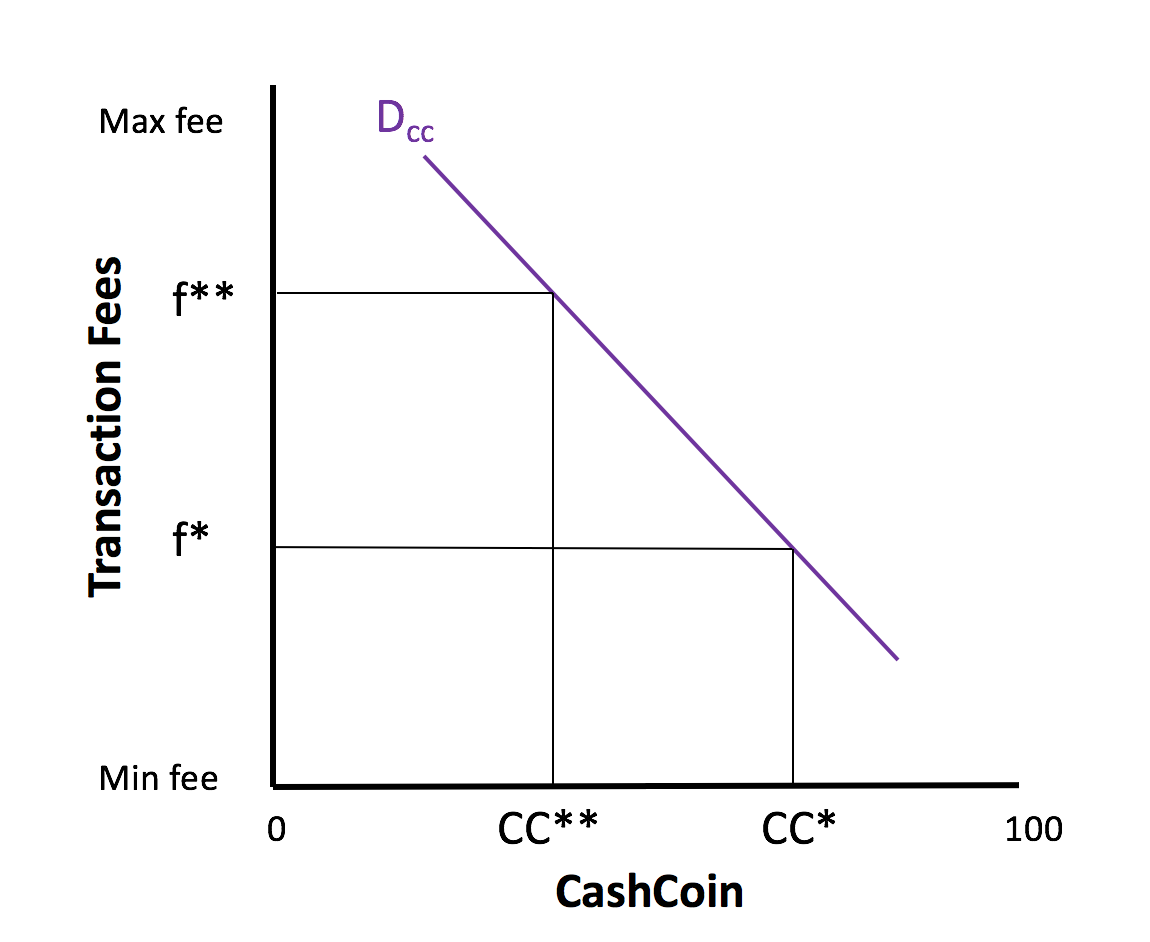
\includegraphics[width=\linewidth]{dcfc}
         \caption{Demand Curve for CashCoin}
         \label{fig21}
     \end{subfigure}
     \vspace{1mm}
     \begin{subfigure}[b]{\linewidth}
         \centering
         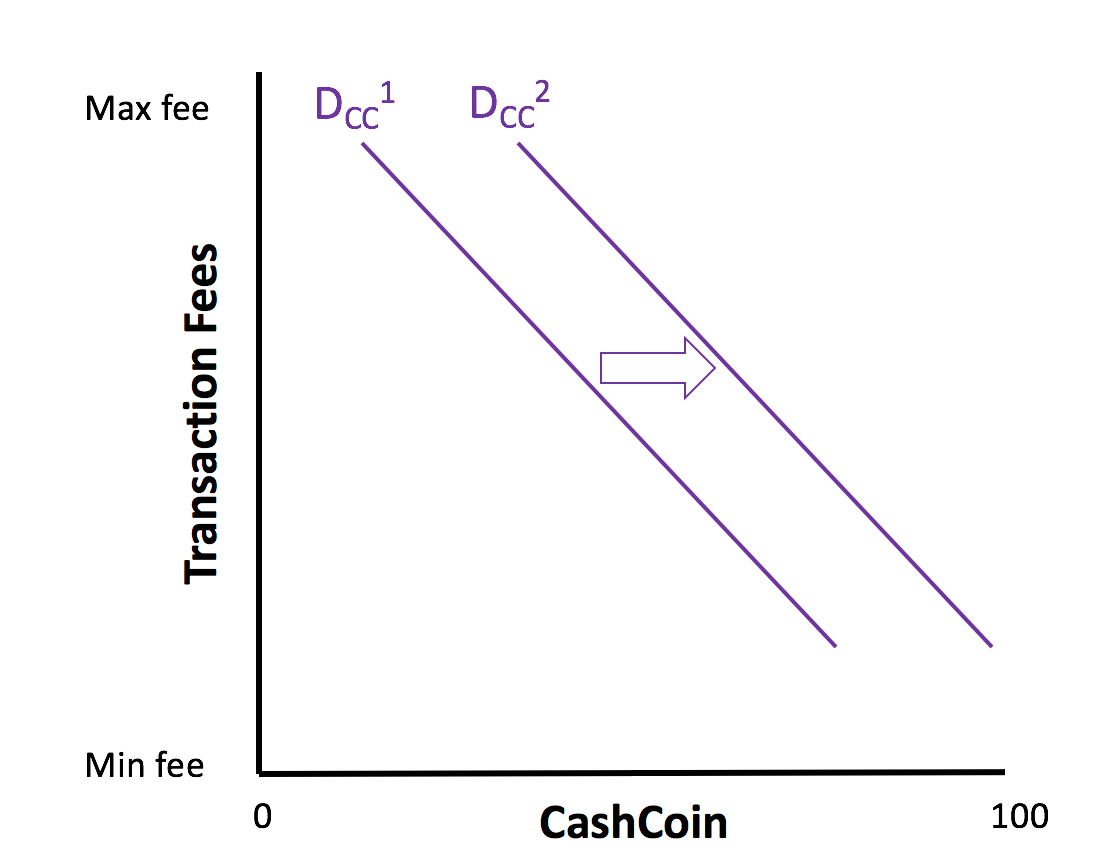
\includegraphics[width=\linewidth]{cidfc}
         \caption{Change in demand for CashCoin}
         \label{fig22}
     \end{subfigure}
        \caption{Dynamics of CashCoin}
        \label{fig2}
\end{figure}


% \begin{figure} [!htbp]
% \centering    
% \subfigure[Demand Curve for CashCoin]{\label{fig31}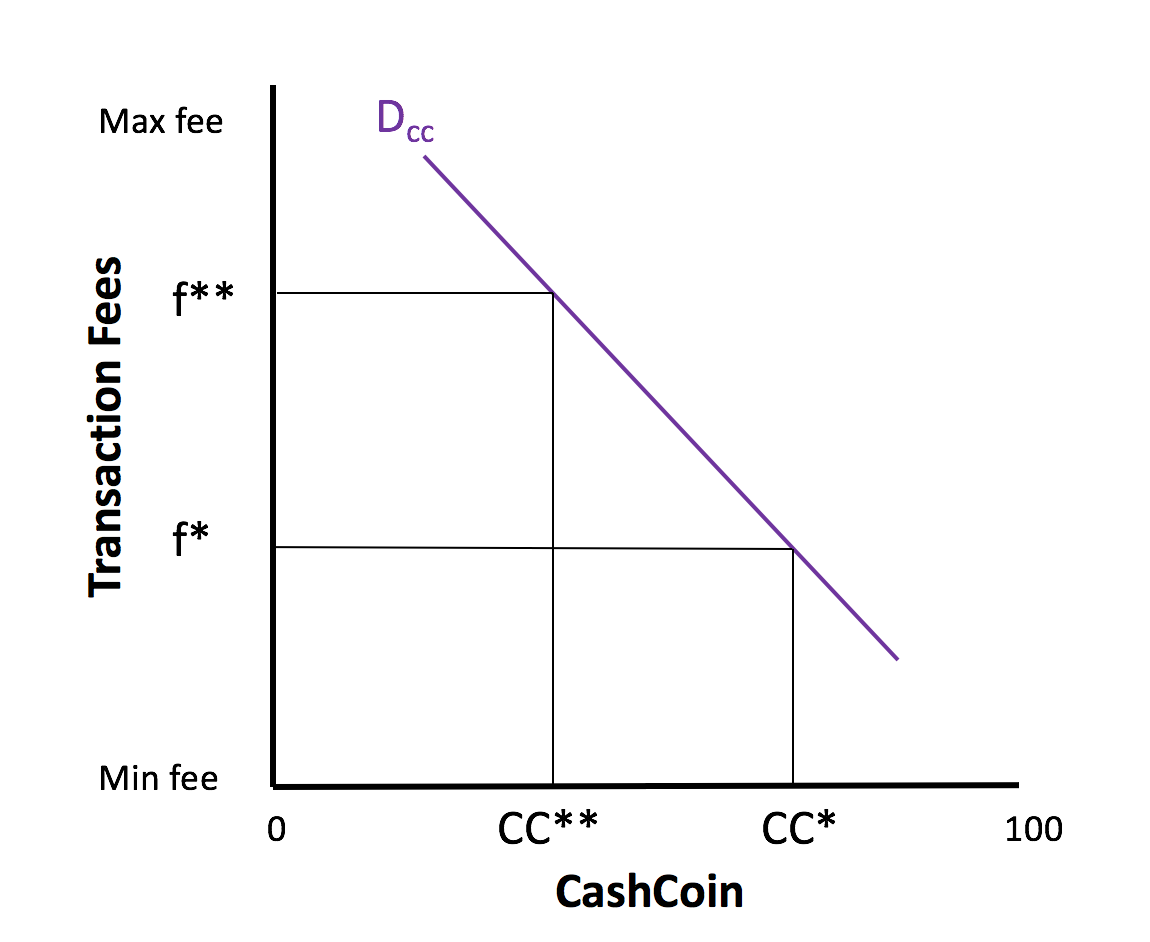
\includegraphics[width=\linewidth]{dcfc.png}}
% \subfigure[Change in demand for CashCoin]{\label{fig32}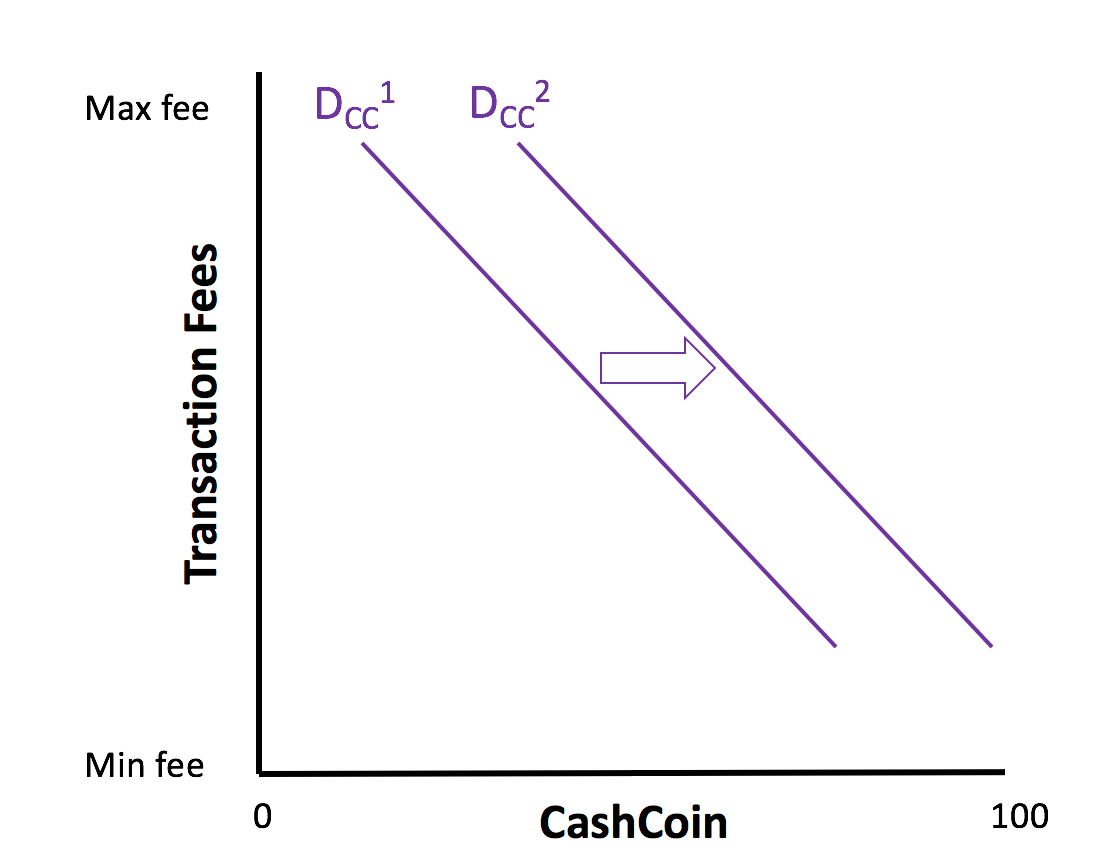
\includegraphics[width=\linewidth]{cidfc.png}}
% \caption{Dynamics of CashCoin}
% \end{figure}

The various sources of demand for CashCoins (transactions, precautionary and speculative) will vary negatively with transaction fees. An additional source of demand for CashCoins is from participants wanting lesser decentralization, faster throughputs and lower fees. Let's label this demand as the higher network performance demand. Lower the fees, higher the demand for CashCoins.

Lets suppose CC** is the total amount of CashCoins at some point in time. I.e., CC** is the supply of CashCoins. Then, the CashCoin market equilibrium will occur at transaction fee f** where the demand meets supply. Now, suppose CashCoin availability increases to CC*, the market equilibrium will occur at transaction fee f* where the demand curve meets the new supply.

\subsubsection{Change in Demand for CashCoin}

Previously, we have identified 4 sources of demands for CashCoins. i) transactions demand, ii) precautionary demand, iii) speculative demand and iv) higher network performance demand. The various sources of demand for CashCoins can change. For example, during festivals in light of higher retail spending, the transaction demand may rise moving the demand curve as shown in the above figure.

\subsubsection{Demand Curve for BondCoin}

The various sources of demand for BondCoins (storage, fees and speculative) will vary positively with transaction fees. An additional source of demand for BondCoins is from participants wanting more decentralization and who do not mind paying higher fees. Let’s label this demand as the higher decentralization demand. Higher the fees, higher the demand for BondCoins.

\begin{figure}
     \centering
     \begin{subfigure}[b]{\linewidth}
         \centering
         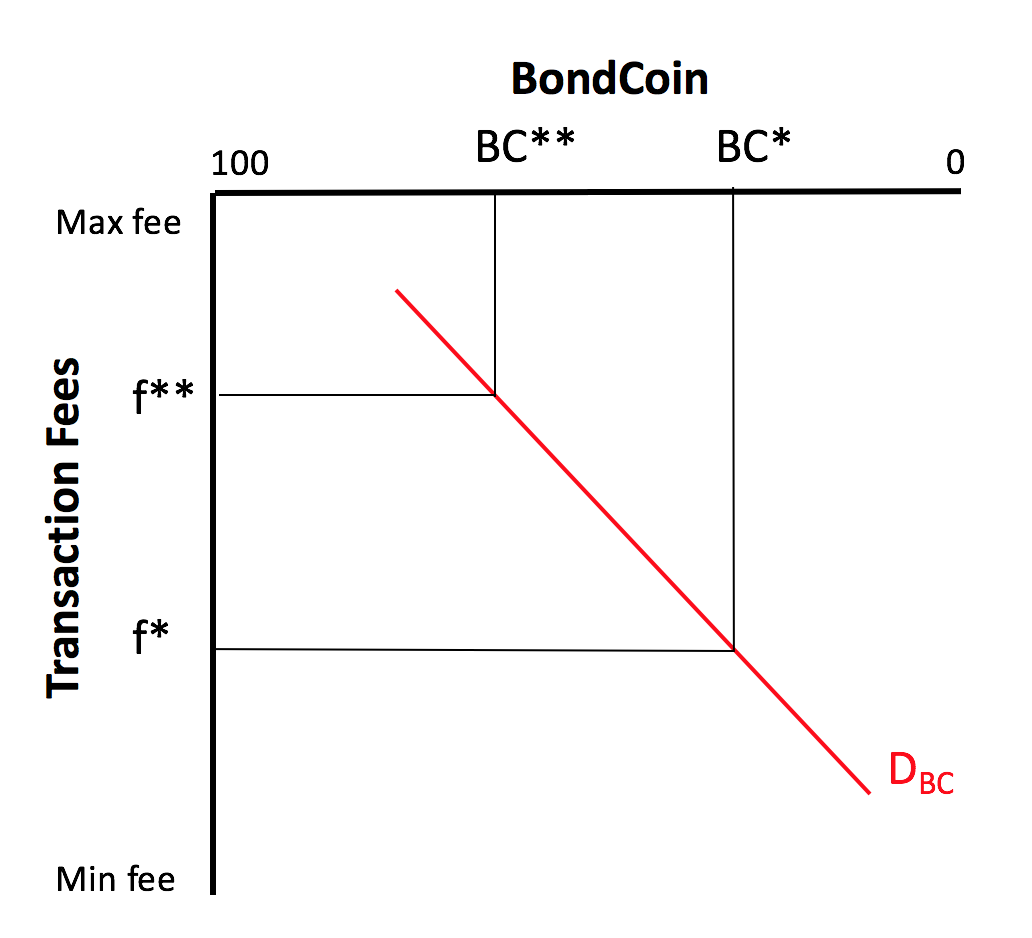
\includegraphics[width=\linewidth]{dcfb}
         \caption{Demand Curve for BondCoin}
         \label{fig31}
     \end{subfigure}
     \vspace{1mm}
     \begin{subfigure}[b]{\linewidth}
         \centering
         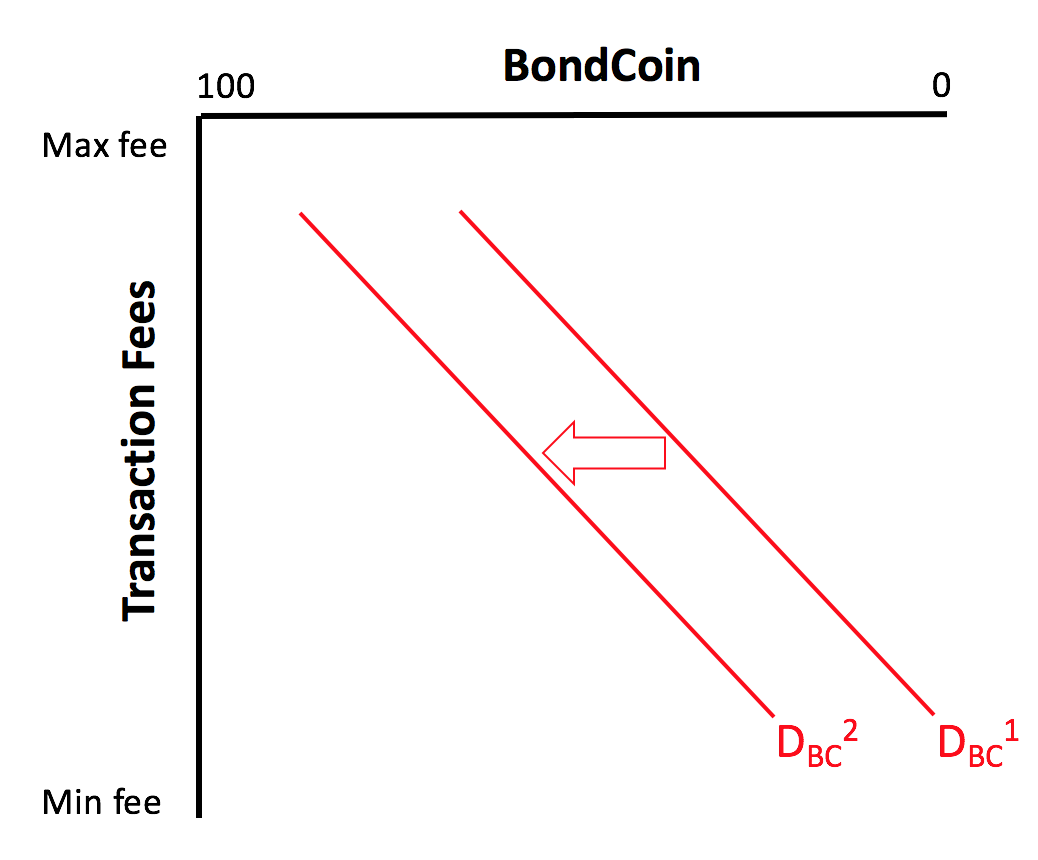
\includegraphics[width=\linewidth]{cidfb}
         \caption{Change in demand for BondCoin}
         \label{fig32}
     \end{subfigure}
        \caption{Dynamics of BondCoin}
        \label{fig3}
\end{figure}

% \begin{figure} [!htbp]
% \centering    
% \subfigure[Demand Curve for BondCoin]{\label{fig33}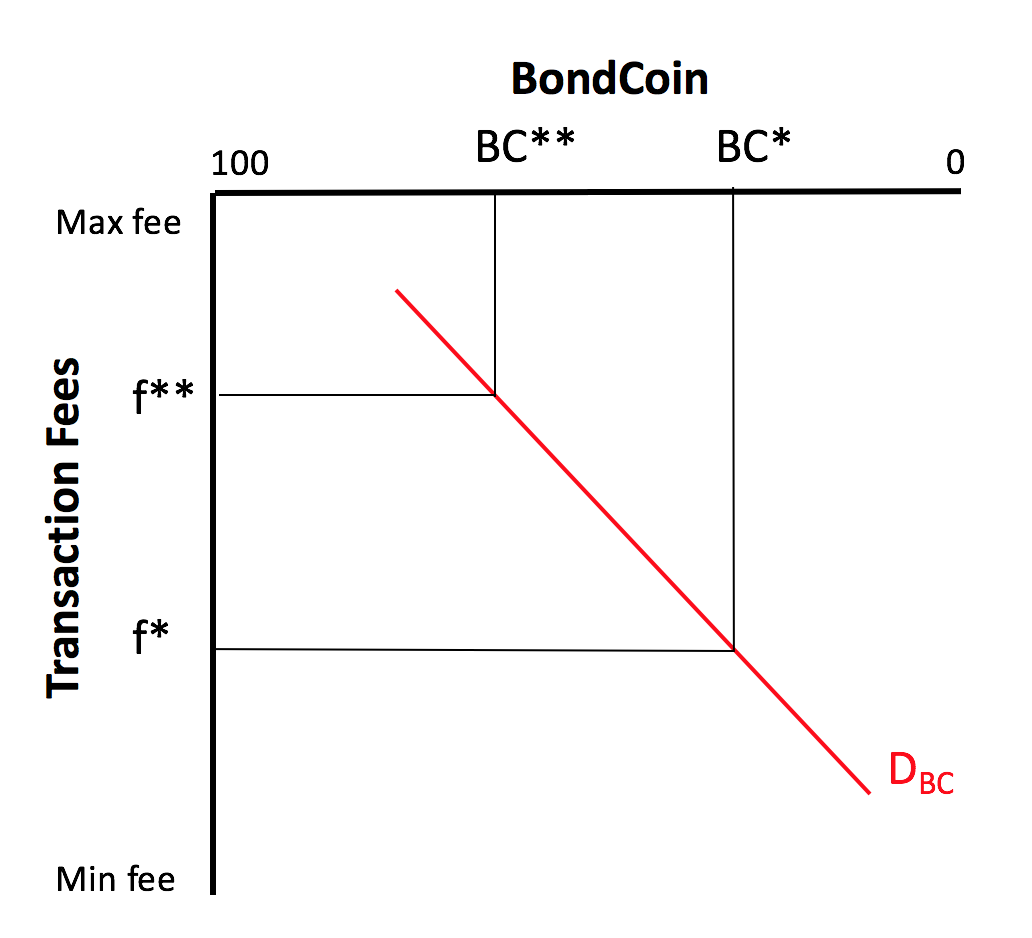
\includegraphics[width=\linewidth]{dcfb.png}}
% \vspace{1cm}
% \subfigure[Change in demand for BondCoin]{\label{fig34}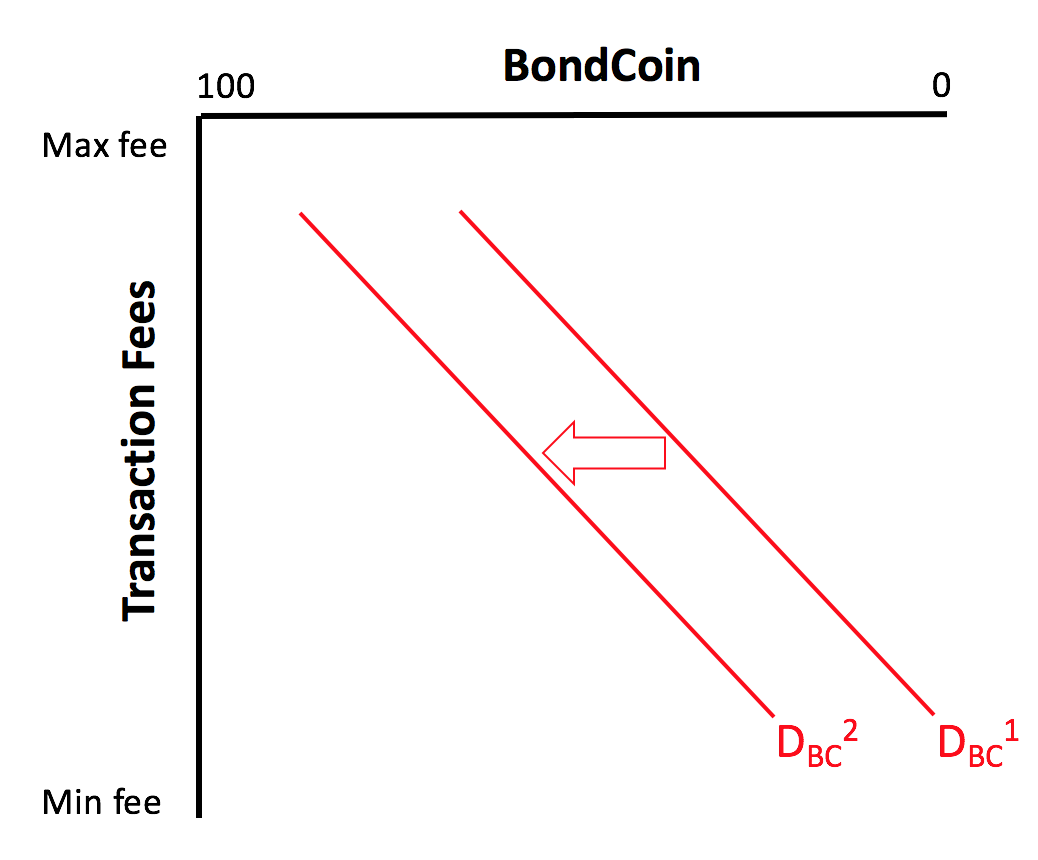
\includegraphics[width=\linewidth]{cidfb.png}}
% \caption{Dynamics of BondCoin}
% \end{figure}

Lets suppose BC* is the total number of BondCoins at some point in time. I.e., BC* is the supply of BondCoins. Then, the BondCoin market equilibrium will occur at transaction fee f* where the demand meets supply. Now, suppose BondCoin availability increases to BC**, the market equilibrium will occur at transaction fee f** where the demand curve meets the new supply.

\subsubsection{Change in Demand for BondCoin}

Previously, we have identified 4 sources of demands for BondCoins. i) storage demand, ii) fees demand, iii) speculative demand and iv) higher decentralization demand. The various sources of demand for BondCoins can change. For example, if the transaction fees increase in anticipation of subdued transaction volumes, the fee demand may rise moving the demand curve as shown in the above figure.

\subsection{The Common Market Equilibrium}

The supply of BondCoins is simply maxCoins - supply of CashCoins. As shown below, it can be represented by a single line. The supply curve intersects with the demand curves of CashCoin and BondCoin at the same point. This is the common market equilibrium for both CashCoins and BondCoins. There is of course a single fee value f for this common market equilibrium.

\begin{figure}[!htbp]
\centering
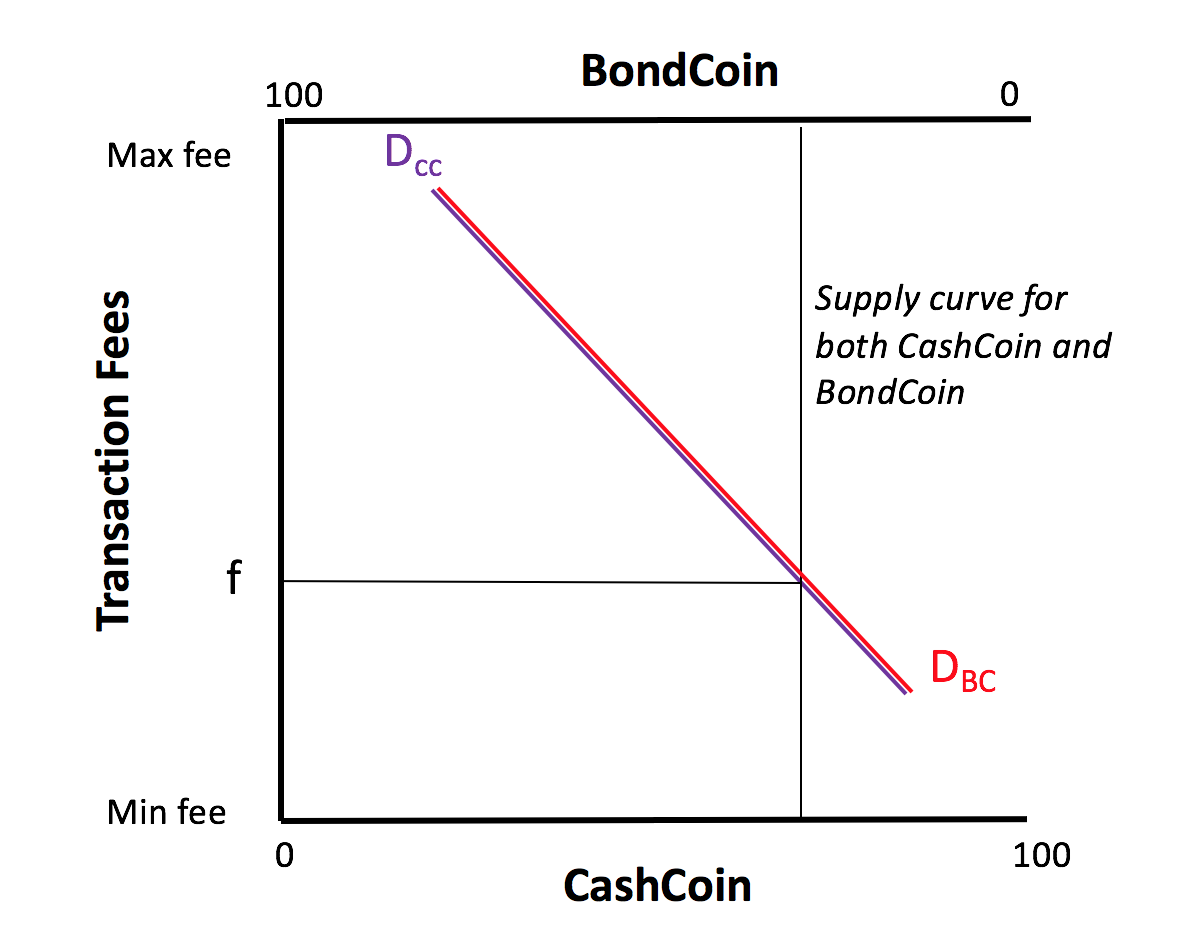
\includegraphics[width=\linewidth]{tcme.png}
\caption{The Common Market Equilibrium}
\label{fig35}
\end{figure}

This common market equilibrium represents the steady state of the system that respects the aggregate demands and supplies for CashCoin and BondCoin. The number of BondCoins at this equilibrium represent the number of validators in the blockchain.


\section{Discussion}

\subsection{Problems in System Design}

Here, we note some of the problems and boundary cases that might occur during the design and execution of the system and we try to give some plausible solutions.

\begin{enumerate}
    \item We know that CashCoins are liquid and can be transferred from one user to another. But, what if a user wants to transfer his voting rights to another user? If this user simply transfers it then he would also have to share the public-private key associated with this coin, but these are digital quantities and can be copied and can lead to the free-rider problem.\\
    Solution : Here, we assume that BondCoins are illiquid and non-transferable. If some user wants to transfer them, then he first has to convert the Coin to CashCoin and send these to the target user who then can convert these back to a BondCoin. This also avoids the free rider problem as when the target user gets his BondCoin, he would also get a new key pair associated with it.
    \item The bond coins are going to be minted using PoW. Once, all the bond coins are minted, the system adopts PoS system. PoW means we are finding some nonce which satisfies some properties, (In case of bitcoin, it had to be less than a given number). But, here the each bond coin is associated with a public and a private key pair which satisfy their own properties. How does the two gets associated?\\
    Solution : Here, the nonce and key-pairs are not related. A user can get a key pair even when PoS has taken over. We use El Gamal Cryptosystem for getting the private-public key pair associated with the BondCoin. This Cryptosystem is based on Elliptic Curve Cryptography (ECDLP) and provides better security with lesser key size. The Base point is common for all users. The private key can be decided by the winner of the current round randomly and based on it a public key can be chosen. But, once its decided, the user cannot change it and has to wait till the BondCoin matures. If he wants to change it then he would have to convert it to CashCoin and then again to BondCoin to choose a new one.
    \item What happens if a user who already owns a BondCoin wins another round while PoW consensus is active?\\
    Solution : If a user wins another round while PoW consensus is active, then he gets to commit that block but the BondCoin that is minted gets added to his account as CashCoin without any penalty. This is done to make sure that each validators has equal voting rights and hence own only one BondCoin with them.
    \item Here we note that PoW algorithm is only for minting bond coins. So, do the users don’t transact till all the bond coins are minted or does the peer minting the next bond coin becomes the leader for that round and commits the block of transactions to the ledger and once all the minting is over, PoS takes over and only those peers can take part in validation who are holding the bond coins?\\
    Solution : Here, we go with the choice that when the PoW consensus is active, the users can still transact and transaction fees are not taken from them. This is done to invite new users to the system and to increase the validators in the system. To incentivise users to participate in the consensus, the BondCoin minted in the current round is paid to the winner of the current round. Note that even after winning once, the users would still want to participate in the consensus to increase the CashCoins in their account.
    \item Each BondCoin comes with a maturity duration d. How is this maturity duration decided? What happens to the keys of the BondCoin once it gets expired and gets converted into CashCoin?\\
    Solution : Currently, this maturity duration is kept as a constant. Eg: 1 month. And, we plan to decide this value emphirically. Each BondCoin comes with a manufacture date, which is stored in the ledger. Once a BondCoin is expired, it gets added as CashCoins to the user account and the keys become useless. This process takes place the first time user transacts after his BondCoin is expired. If he tries to vote using the old keys then his vote is discarded during the expiration check phase.
    \item Since, the CashCoins are not converted automatically to BondCoins, what happens when there is no BondCoin left in the system?\\
    The situation where no BondCoins are left in the system is hard to occur. As the BondCoins in the system decrease, the transaction fees would decrease. In this case, automatically the demand for BondCoins would increase as the few users who are owners of the last few BondCoin would enjoy more shares of the transaction fees by themselves. But, no BondCoin situation can occur only when the last of BondCoins also got matured automatically and no other user converted their CashCoin into a BondCoin before their expiration which would bring the system to a standstill. If there are no BondCoin in the system then there would be no validators in the system and no user would be able to transact and hence the CashCoins in their account would become useless. In this unlikely situation, we suggest that the PoW system is restarted so that the BondCoins in the system can be increased and users can enjoy transactions without paying the fees and do not have to leave the system.
    \item Why is there a penalty for converting BondCoin to CashCoin? How is its amount fixed?\\
    Solution : The BondCoin is like a contract given to user to participate in the validation process during its maturity period. Its like a fixed deposit done in bank, on which you get the interest during the period but you can use the money only after it matures, if you take the money out before it matures then you have to pay a penalty. In a similar way, this penalty is imposed on those users who want to do away with their responsibility of participating in the validation process. The amount is fixed based on the number of BondCoins currently in the system. More the number of BondCoins, more the penalty.

\end{enumerate}

\subsection{Plausible attacks}

Here, we assume that the block has been prepared and validators are decided, we only need to consider attacks that can be made while committing this block to the ledger.

\begin{enumerate}
    \item Adversary can be the owner of majority of bond coins. Adversary can make multiple accounts with only enough cash coin to convert them into bond coins.
    \item If in response to above, the bond coins are made larger in number then network attacks would be easier. Adversary may be able to slow down the network or partition some nodes.
    \item Instead of buying the bond coins itself, adversary may hack prominent accounts holding bond coins. It's useful as they are gonna be valid for duration d.
\end{enumerate}

\section{Distributed Algorithm}

\subsection{Assumptions}

We take the following assumptions for our distributed system :

\begin{itemize}
    \item Each user has a unique id
    \item Each user knows other users
    \item Each user is a node in itself
    \item More than 2/3rd of the users (or specifically the committee members) are honest (non-faulty and form the largest sub) in the system (non-faulty)
    \item New requests for bond coin keep coming in
    \item Each user has a unique public address known to other user while its active
    \item Asynchronous system (Network Faults can happen)
    \item Eventually synchronous system (Eventually all network faults would be resolved)
    \item Reliable connection
    \item Each function is executed atomically
\end{itemize}

\subsection{Abbreviations}

Following are the abbreviations used to denote some fields and classes :

\begin{itemize}
    \item id = User's ID
	\item mt = Transaction Type
	\item sid = Sender's ID
	\item rid = Reciever's ID
	\item t = Timestamp, can also be the id of the last block seen by the user to avoid time conflicts
	\item cc = CashCoin
	\item bc = BondCoin
	\item pk = Public Key of a user
	\item sk = Secret Key / Private Key of a user
	\item val = Transaction amount value that a user wants to send to another user
	\item h = hash obtained on applying a verifiable random function on the message using sk
	\item p = proof for verifying the hash of a message using that user's pk
	\item pa = public address for committee to communicate with this node during consensus
	\item fb = First Block in which a user starts giving consensus
	\item lb = Last Block after which a user stops giving consensus
	\item cps = Cryptocurrency Participation Score
	\item k = The number of blocks till which a transaction is valid. If a transaction is more than 
\end{itemize}

\subsection{Message Types}

Following messages will be exchanged in the system :

\begin{enumerate}
    \item Transfer : Message gossiped by the a node with id sid to send val amount of cashcoins to a node with id rid at timestamp t.
    \begin{verbatim}
Message Transfer
{
    mt
    sid
    rid
    val
    tc
    t
    h
    p
}
    \end{verbatim}
    \item RequestBC : Message requesting to convert cashcoin to bondcoin and become a member of the committee.
    \begin{verbatim}
Message RequestBC
{
    mt
    sid
    pa
    tc
    t
    h
    p
}
    \end{verbatim}
    \item RequestCC : Message requesting to convert bondcoin to cashcoin before maturity.
    \begin{verbatim}
Message RequestCC
{
    mt
    sid
    tc
    t
    h
    p
}
    \end{verbatim}
    \item ChangePK : Message requesting to change pk.
    \begin{verbatim}
Message ChangePK
{
    mt
    sid
    pk // New Public Key
    tc
    t
    h
    p
}
    \end{verbatim}
    \item Join : Message requesting to join the system as a new user. The new id would be mentioned in the next few blocks as confirmation.
    \begin{verbatim}
Message Join
{
    mt
    pk
    tc
    t
    h
    p
}
    \end{verbatim}
    \item BlockCommit : Message broadcasted to give info about a new block.
    \begin{verbatim}
Message BlockCommit
{
    mt  // type of message
    sid // sender id
    block // block list element
    h // hash
    p // proof
}
    \end{verbatim}
\end{enumerate}

\subsection{Variables stored at each node}

\begin{enumerate}
    \item pk = Public Key : This key is advertised by the node so that other nodes can use it to verify its messages, its unique to a node and used to index the its information in the database.
    \item sk = Private Key : This is the only private state of the node (same as in algorand) and is used to sign the messages sent by it.
    \item cmq = CommMemm : Queue of members of the committee arranged according to the expiration of their voting rights. The new committee members are added at the tail of this queue and oldest committee members at the head of the queue are popped as their rights expire. When a new committee member is added, they would be pushed to the tail of the queue.
    \item ll = Ledger : List of blocks of transactions that have been committed till now.
    \item ssd = SystemState : Dictionary of users of the system with their public ids as the key and the amount of ccs they have as the value. Additional information can also be kept in the structure to calculate the likelihood of that user being selected in the committee if the user contests for voting rights. These information include the number of transactions he has done in the past
    \item maxid (for ca only) : denotes the number of unique ids already given away to nodes starting at 0.
\end{enumerate}

#A user might exploit the number of transactions to gain voting rights but in the process he would have to pay the transaction fees for each transaction. Also, this is the hard work the adversary has to do for just one user but he would be in a position to attack only if he has access to half of the committee members.
#As the ca keeps track of the state of the system and knows the committee, it would know if a node requesting to leave the system is part of the committee or not and hence, can accordingly approve the request.
#For nodes, not participating in the consensus whose ccs are freezed, a penalty may be applicable for storage of the ccs, to discourage such events.
#ssd values are objects having following fields :
    active : indicating whether joined in the network
    id : unique id given by the ca on joining the network
    cc : amt of cashcoins the node has
    member : indicating whether a member of committee or not
#Transactions also contain the members which are losing their rights and the new members that are going to be added, accordingly their ccoins value shall be updated in the network
#The committee members must agree with each other, hence while joining the committee they can compare their states with older members of the committee. <Lemma> The state of any committee member at time t can be obtained by applying the transactions change on any state at time tcap even though the present committee member might not be a part of previous committee. </Lemma> can be proved as outgoing cms must have the same state as incoming cms, can put induction to prove. Instead, can also put this check while selecting new committee members and filter out those who don't have the same state.
#The other members of the system can also verify to whether they have the same state as the current committee members.
#Each user would be listening to the transactions being broadcasted and the blocks being committed, so that once a user has got acceptance in a block, he can start committing
#To change the public key, the node needs to send the corresponding request to the ca who then needs to forward it to the committee as a transaction. It needs to check first that the key is unique.
#Functions can run in parallel threads
#Transaction Functions :
    The transaction fees is decided by a function of committee size (this means everybody must know who all are in the committee). It satisfies following conditions :
    1) It is positive for all possible committee sizes.
    2) It has a maximum value at anchor point. This is the point which define the value of the transactions fees and committee size when the system is in stable state.
    3) The function must be a strictly increasing function below the anchor point and strictly decreasing function above the anchor point.
#This anchor point may be adjusted during the execution. Also, it doesn't matter what is the actual penalty. Since, it is going to be equally distributed between the members.
We choose functions of the form f=$x^n*e^-x$ whose derivative has n solutions with n-1 0s and 1 non zero value. x = 0 or x = n are the points and max value is $n^n*e^-n$. Therefore, if we want to have anchor point at m (stable committee size) and transaction fees at p (proportion of transaction amount deducted as fees) then we can convert this function the following way.
To set the anchor point at m, substite x = $x'*n/30$ f' = $(x'*n/30)^n*e^-(x'*n/30)$ . To set max value at p, substitue f'' = $f'*p/(n^n*e^-n)$.
Note that as the value of n increases the peak becomes sharper and sharper
#Flaw : If we are doing a majority, should those who are not part of majority also earn from the transaction fees, if not then it might be inconsistent.
#Flaw : If there is no consensus, then do the voters agree on empty block like in algorand, in that case do we allow new users to come and old users to retire? If new users are put in queue then do we allow them to participate from the next round itself or do we wait for some time or randomly pick them up?

VerifyMessage(m = message, pk = public key, e = encryption, p = proof) :
    Use pk and p to verify whether e is a valid encryption of m
    If it is valid :
        return true
    Else :
        return false

% SendMessage(m = message, j = node) :
%     e, p = Encrypt(m#t, sk)
%     Send 
EncryptMessage(m = message, t) :
    e, p = encryption(m#t, sk)
    return e,p
    
SendCommittee(m=message) :
    e,p = Encrypt(m,sk)
    For each member in cmq :
        Send m to member
        
Broadcast(m=message) :
    for all pk in ssd.keys :
        If ssd[pk].active = 1 :
            Send m to ssd[pk].id
    
Consul agent : Special node for tracking the nodes which are joined in the system and which are dead and finding each other. The consul agent acts like a normal node except it can never participate in the consensus. But, it does keep track of the state of the system and the committee members like every other node. It does not have any cc or bc allotted to it.

On recieving Join(pk = Public Key , e(sk, t) = Encryption of t using sk(secret key) , p = proof(sk, t), t = timestamp when the message was sent) from node i :
    // ca verifies whether the message is valid by calling VerifyMessage()
    treply = current time
    
    // If message verification fails
    If VerifyMessage(t, pk, e, p) = False :
        mreply = "Signature cannot be verified"
        Send RejectJoin(mreply, ereply, preply, treply) to j
    
    // If the node is already joined
    If pk in ssd.keys and ssd[pk].active = true :
        mreply = "Node already joined with id " + ssd[pk].id
        ereply, preply = EncryptMessage(mreply, treply)
        Send RejectJoin(mreply, ereply, preply, treply) to j
    
    // The node is new, pk is unique
    // The ca needs to send the request as a transaction to the committee and only after it gets committed, the new node can be added after which the ca can broadcast its id to all the nodes. After sending the message to all the members, if the ca doesn't recieve committed within some blocks(based on some maximum time delta between sending a transaction and getting it committed) then it replies the node the transaction is failed otherwise it sends a success message to it
    atomic {
            tempid = maxid
            maxid++
        }
    mreply = "Add a new node with public key "+pk+" id "+tempid
    ereply,preply = EncryptMessage(mreply, treply)
    mreply = AddNode(mreply, ereply, preply, treply)
    SendComittee(mreply)
    
    If ca sees the corresponding transaction getting committed within some blocks :
        ssd[pk] = {active = 1, id = tempid, cc = 0, member = 0}
        mreply = "Node accepted to join with id " + ssd[pk].id
        ereply, preply = EncryptMessage(mreply, treply)
        Send AcceptJoin(mreply, ereply, preply, treply) to j
        
        tbroadcast = current time
        mbroadcast = "New node accepted to join with id "+ssd[pk].id+" and pk "+pk
        ebroadcast, pbroadcast = EncryptMessage(mbroadcast, tbroadcast)
        mbroadcast = AddNodeBroadcast(mbroadcast, ebroadcast, pbroadcast, tbroadcast)
        Broadcast(mbroadcast)
    
    Else :
        mreply = "Committee didn't accept"
        ereply, preply = EncryptMessage(mreply, treply)
        Send RejectJoin(mreply, ereply, preply, treply) to j

\section{Conclusion and Future Works}

In this report, we saw how the number of validators for a POS system can be dynamic and may be determined by the market parameters. The POS systems were better than POW systems because they don't waste computational power in redundant tasks but POS systems itself has some drawbacks. The proposed system tries to solve some of these drawbacks. The crux of the proposed system lies in the fact that all the validators are given equal voting rights so that adversary is also ripped off of the probabilistic advantage of gaining the control of the system which is prevalent in the recently proposed systems such as Algorand. In this system, gaining half the currency of the system is not enough for the adversary. He must have control over more than half of the BondCoins i.e. more than half of the computation power. And, as these BondCoins come with an expiry, the task of the adversary becomes more difficult.

In future we would like to achieve the following objectives :
\begin{enumerate}
    \item We would like to explore how the system is affected if the maturity duration of a BondCoin is variable
    \item We would like to devise a method to ensure that a minimum number of validators are always there in the network at a given point of time
    \item We would like to explore how the system is affected if the BondCoin is also quantized. For eg : a group of users can combine their CashCoins to get one BondCoin. What would be the final vote of such a group of users?
    \item Till now, we have assumed that all the validators remain active all the time. We would like to explore what happens if some of the validators crash or go offline.
    \item We would like to tackle the geographical scalability of POS protocols and devise a solution for it.
    \item We would like to implement a prototype of the above proposed system and run benchmark tests on it.
    \item We would like to explore how charging fees for conversion of CashCoin to BondCoin affects the economy of the system.
\end{enumerate}


\section{References}

\begin{enumerate}
    \item S. Nakamoto, Bitcoin: A Peer-to-Peer Electronic Cash System, 2008.
    \item S. Liu, P. Viotti, C. Cachin, V. Quéma, M. Vukolic, "XFT: practical fault tolerance beyond crashes", Proc. 12th USENIX OSDI, 2016.
    \item Y. Gilad, R. Hemo, S. Micali, G. Vlachos, N. Zeldovich, "Algorand: Scaling Byzantine Agreements for Cryptocurrencies", Cryptology ePrint Archive Report 2017/454, 2017.
    \item https://en.wikipedia.org/wiki/State\_machine\_replication
    \item https://en.wikipedia.org/wiki/Blockchain
    \item https://medium.com/@deshpande.pralhad/a-proof-of-stake-blockchain-with-two-native-asset-types-35f643bb3ff3
    \item https://open.lib.umn.edu/principleseconomics/chapter/25-2-demand-supply-and-equilibrium-in-the-money-market/
    \item https://medium.com/coinmonks/understanding-proof-of-stake-the-nothing-at-stake-theory-1f0d71bc027
    \item https://lisk.io/academy/blockchain-basics/how-does-blockchain-work/proof-of-stake
\end{enumerate}

\section{Authors and Affiliations}

Each author must be defined separately for accurate metadata identification. Multiple authors may share one affiliation. Authors' names should not be abbreviated; use full first names wherever possible. Include authors' e-mail addresses whenever possible.

Grouping authors' names or e-mail addresses, or providing an ``e-mail alias,'' as shown below, is not acceptable:
\begin{verbatim}
  \author{Brooke Aster, David Mehldau}
  \email{dave,judy,steve@university.edu}
  \email{firstname.lastname@phillips.org}
\end{verbatim}

The \verb|authornote| and \verb|authornotemark| commands allow a note to apply to multiple authors --- for example, if the first two authors of an article contributed equally to the work. 

If your author list is lengthy, you must define a shortened version of the list of authors to be used in the page headers, to prevent overlapping text. The following command should be placed just after the last \verb|\author{}| definition:
\begin{verbatim}
  \renewcommand{\shortauthors}{McCartney, et al.}
\end{verbatim}
Omitting this command will force the use of a concatenated list of all of the authors' names, which may result in overlapping text in the page headers.

The article template's documentation, available at  \url{https://www.acm.org/publications/proceedings-template}, has a complete explanation of these commands and tips for their effective use.

\section{Rights Information}

Authors of any work published by ACM will need to complete a rights form. Depending on the kind of work, and the rights management choice made by the author, this may be copyright transfer, permission, license, or an OA (open access) agreement.

Regardless of the rights management choice, the author will receive a copy of the completed rights form once it has been submitted. This form contains \LaTeX\ commands that must be copied into the source document. When the document source is compiled, these commands and their parameters add formatted text to several areas of the final document:
\begin{itemize}
\item the ``ACM Reference Format'' text on the first page.
\item the ``rights management'' text on the first page.
\item the conference information in the page header(s).
\end{itemize}

Rights information is unique to the work; if you are preparing several works for an event, make sure to use the correct set of commands with each of the works.

\section{CCS Concepts and User-Defined Keywords}

Two elements of the ``acmart'' document class provide powerful taxonomic tools for you to help readers find your work in an online search. 

The ACM Computing Classification System --- \url{https://www.acm.org/publications/class-2012} --- is a set of classifiers and concepts that describe the computing discipline. Authors can select entries from this classification system, via \url{https://dl.acm.org/ccs/ccs.cfm}, and generate the commands to be included in the \LaTeX\ source. 

User-defined keywords are a comma-separated list of words and phrases of the authors' choosing, providing a more flexible way of describing the research being presented.

CCS concepts and user-defined keywords are required for all short- and full-length articles, and optional for two-page abstracts. 

\section{Sectioning Commands}

Your work should use standard \LaTeX\ sectioning commands: \verb|section|, \verb|subsection|, \verb|subsubsection|, and \verb|paragraph|. They should be numbered; do not remove the numbering from the commands. 

Simulating a sectioning command by setting the first word or words of a paragraph in boldface or italicized text is {\bf not allowed.}

\section{Tables}

The ``\verb|acmart|'' document class includes the ``\verb|booktabs|'' package --- \url{https://ctan.org/pkg/booktabs} --- for preparing high-quality tables. 

Table captions are placed {\it above} the table.

Because tables cannot be split across pages, the best placement for them is typically the top of the page nearest their initial cite.  To ensure this proper ``floating'' placement of tables, use the environment \textbf{table} to enclose the table's contents and the table caption.  The contents of the table itself must go in the \textbf{tabular} environment, to be aligned properly in rows and columns, with the desired horizontal and vertical rules.  Again, detailed instructions on \textbf{tabular} material are found in the \textit{\LaTeX\ User's Guide}.

Immediately following this sentence is the point at which Table~\ref{tab:freq} is included in the input file; compare the placement of the table here with the table in the printed output of this document.

\begin{table}
  \caption{Frequency of Special Characters}
  \label{tab:freq}
  \begin{tabular}{ccl}
    \toprule
    Non-English or Math&Frequency&Comments\\
    \midrule
    \O & 1 in 1,000& For Swedish names\\
    $\pi$ & 1 in 5& Common in math\\
    \$ & 4 in 5 & Used in business\\
    $\Psi^2_1$ & 1 in 40,000& Unexplained usage\\
  \bottomrule
\end{tabular}
\end{table}

To set a wider table, which takes up the whole width of the page's live area, use the environment \textbf{table*} to enclose the table's contents and the table caption.  As with a single-column table, this wide table will ``float'' to a location deemed more desirable. Immediately following this sentence is the point at which Table~\ref{tab:commands} is included in the input file; again, it is instructive to compare the placement of the table here with the table in the printed output of this document.

\begin{table*}
  \caption{Some Typical Commands}
  \label{tab:commands}
  \begin{tabular}{ccl}
    \toprule
    Command &A Number & Comments\\
    \midrule
    \texttt{{\char'134}author} & 100& Author \\
    \texttt{{\char'134}table}& 300 & For tables\\
    \texttt{{\char'134}table*}& 400& For wider tables\\
    \bottomrule
  \end{tabular}
\end{table*}

\section{Math Equations}
You may want to display math equations in three distinct styles:
inline, numbered or non-numbered display.  Each of
the three are discussed in the next sections.

\subsection{Inline (In-text) Equations}
A formula that appears in the running text is called an
inline or in-text formula.  It is produced by the
\textbf{math} environment, which can be
invoked with the usual \texttt{{\char'134}begin\,\ldots{\char'134}end}
construction or with the short form \texttt{\$\,\ldots\$}. You
can use any of the symbols and structures,
from $\alpha$ to $\omega$, available in
\LaTeX~\cite{Lamport:LaTeX}; this section will simply show a
few examples of in-text equations in context. Notice how
this equation:
\begin{math}
  \lim_{n\rightarrow \infty}x=0
\end{math},
set here in in-line math style, looks slightly different when
set in display style.  (See next section).

\subsection{Display Equations}
A numbered display equation---one set off by vertical space from the
text and centered horizontally---is produced by the \textbf{equation}
environment. An unnumbered display equation is produced by the
\textbf{displaymath} environment.

Again, in either environment, you can use any of the symbols
and structures available in \LaTeX\@; this section will just
give a couple of examples of display equations in context.
First, consider the equation, shown as an inline equation above:
\begin{equation}
  \lim_{n\rightarrow \infty}x=0
\end{equation}
Notice how it is formatted somewhat differently in
the \textbf{displaymath}
environment.  Now, we'll enter an unnumbered equation:
\begin{displaymath}
  \sum_{i=0}^{\infty} x + 1
\end{displaymath}
and follow it with another numbered equation:
\begin{equation}
  \sum_{i=0}^{\infty}x_i=\int_{0}^{\pi+2} f
\end{equation}
just to demonstrate \LaTeX's able handling of numbering.

\section{Figures}

The ``\verb|figure|'' environment should be used for figures. One or more images can be placed within a figure. If your figure contains third-party material, you must clearly identify it as such, as shown in the example below.
\begin{figure}[h]
  \centering
  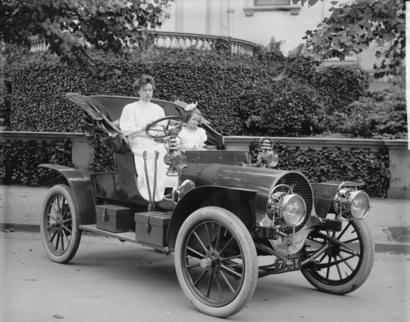
\includegraphics[width=\linewidth]{sample-franklin}
  \caption{1907 Franklin Model D roadster. Photograph by Harris \& Ewing, Inc. [Public domain], via Wikimedia Commons. (\url{https://goo.gl/VLCRBB}).}
  \Description{The 1907 Franklin Model D roadster.}
\end{figure}

Your figures should contain a caption which describes the figure to the reader. Figure captions go below the figure. Your figures should {\bf also} include a description suitable for screen readers, to assist the visually-challenged to better understand your work.

Figure captions are placed {\it below} the figure.

\subsection{The ``Teaser Figure''}

A ``teaser figure'' is an image, or set of images in one figure, that are placed after all author and affiliation information, and before the body of the article, spanning the page. If you wish to have such a figure in your article, place the command immediately before the \verb|\maketitle| command:
\begin{verbatim}
  \begin{teaserfigure}
    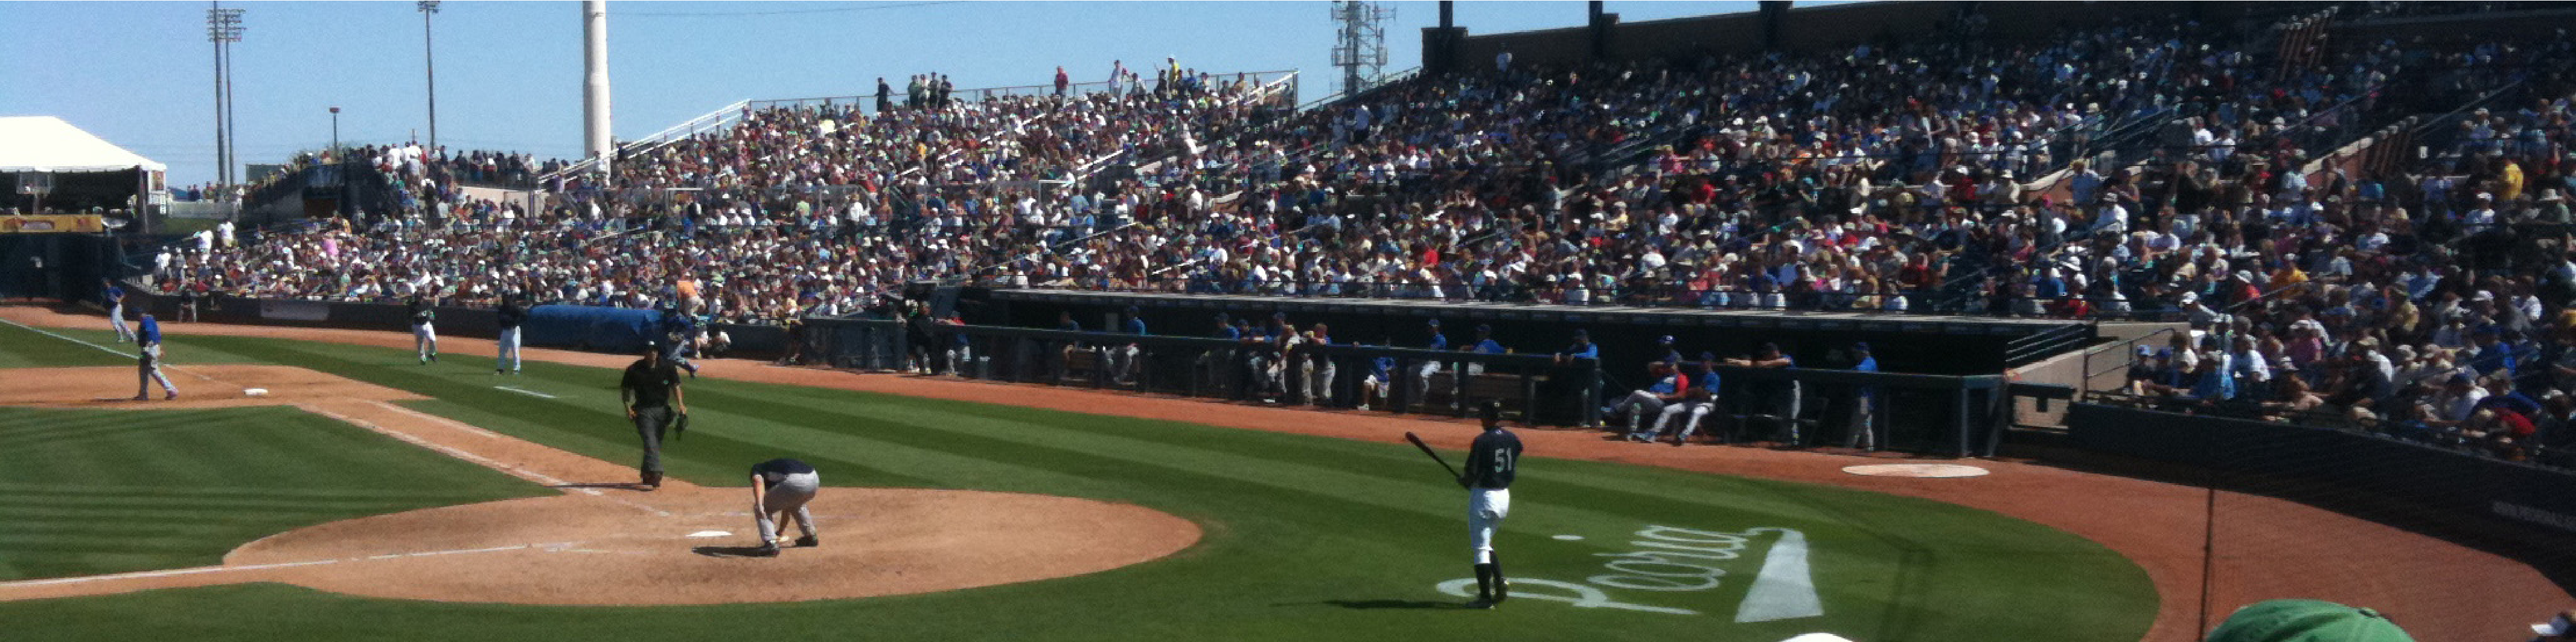
\includegraphics[width=\textwidth]{sampleteaser}
    \caption{figure caption}
    \Description{figure description}
  \end{teaserfigure}
\end{verbatim}

\section{Citations and Bibliographies}

The use of \BibTeX\ for the preparation and formatting of one's references is strongly recommended. Authors' names should be complete --- use full first names (``Donald E. Knuth'') not initials (``D. E. Knuth'') --- and the salient identifying features of a reference should be included: title, year, volume, number, pages, article DOI, etc. 

The bibliography is included in your source document with these two commands, placed just before the \verb|\end{document}| command:
\begin{verbatim}
  \bibliographystyle{ACM-Reference-Format}
  \bibliography{bibfile}
\end{verbatim}
where ``\verb|bibfile|'' is the name, without the ``\verb|.bib|'' suffix, of the \BibTeX\ file.

Citations and references are numbered by default. A small number of ACM publications have citations and references formatted in the ``author year'' style; for these exceptions, please include this command in the {\bf preamble} (before ``\verb|\begin{document}|'') of your \LaTeX\ source: 
\begin{verbatim}
  \citestyle{acmauthoryear}
\end{verbatim}

Some examples.  A paginated journal article \cite{Abril07}, an enumerated journal article \cite{Cohen07}, a reference to an entire issue \cite{JCohen96}, a monograph (whole book) \cite{Kosiur01}, a monograph/whole book in a series (see 2a in spec. document)
\cite{Harel79}, a divisible-book such as an anthology or compilation \cite{Editor00} followed by the same example, however we only output the series if the volume number is given \cite{Editor00a} (so Editor00a's series should NOT be present since it has no vol. no.),
a chapter in a divisible book \cite{Spector90}, a chapter in a divisible book in a series \cite{Douglass98}, a multi-volume work as book \cite{Knuth97}, an article in a proceedings (of a conference, symposium, workshop for example) (paginated proceedings article) \cite{Andler79}, a proceedings article with all possible elements \cite{Smith10}, an example of an enumerated proceedings article \cite{VanGundy07}, an informally published work \cite{Harel78}, a doctoral dissertation \cite{Clarkson85}, a master's thesis: \cite{anisi03}, an online document / world wide web resource \cite{Thornburg01, Ablamowicz07, Poker06}, a video game (Case 1) \cite{Obama08} and (Case 2) \cite{Novak03} and \cite{Lee05} and (Case 3) a patent \cite{JoeScientist001}, work accepted for publication \cite{rous08}, 'YYYYb'-test for prolific author \cite{SaeediMEJ10} and \cite{SaeediJETC10}. Other cites might contain 'duplicate' DOI and URLs (some SIAM articles) \cite{Kirschmer:2010:AEI:1958016.1958018}. Boris / Barbara Beeton: multi-volume works as books \cite{MR781536} and \cite{MR781537}. A couple of citations with DOIs: \cite{2004:ITE:1009386.1010128,Kirschmer:2010:AEI:1958016.1958018}. Online citations: \cite{TUGInstmem, Thornburg01, CTANacmart}.

\section{Acknowledgments}

Identification of funding sources and other support, and thanks to individuals and groups that assisted in the research and the preparation of the work should be included in an acknowledgment section, which is placed just before the reference section in your document. 

This section has a special environment:
\begin{verbatim}
  \begin{acks}
  ...
  \end{acks}
\end{verbatim}
so that the information contained therein can be more easily collected during the article metadata extraction phase, and to ensure consistency in the spelling of the section heading. 

Authors should not prepare this section as a numbered or unnumbered {\verb|\section|}; please use the ``{\verb|acks|}'' environment.

\section{Appendices}

If your work needs an appendix, add it before the ``\verb|\end{document}|'' command at the conclusion of your source document. 

Start the appendix with the ``\verb|appendix|'' command:
\begin{verbatim}
  \appendix
\end{verbatim}
and note that in the appendix, sections are lettered, not numbered. This document has two appendices, demonstrating the section and subsection identification method.

\section{SIGCHI Extended Abstracts}

The ``\verb|sigchi-a|'' template style (available only in \LaTeX\ and not in Word) produces a landscape-orientation formatted article, with a wide left margin. Three environments are available for use with the ``\verb|sigchi-a|'' template style, and produce formatted output in the margin:
\begin{itemize}
\item {\verb|sidebar|}:  Place formatted text in the margin.
\item {\verb|marginfigure|}: Place a figure in the margin.
\item {\verb|margintable|}: Place a table in the margin.
\end{itemize}

%
% The acknowledgments section is defined using the "acks" environment (and NOT an unnumbered section). This ensures
% the proper identification of the section in the article metadata, and the consistent spelling of the heading.
\begin{acks}
To Robert, for the bagels and explaining CMYK and color spaces.
\end{acks}

%
% The next two lines define the bibliography style to be used, and the bibliography file.
\bibliographystyle{ACM-Reference-Format}
\bibliography{sample-base}

% 
% If your work has an appendix, this is the place to put it.
\appendix

\section{Research Methods}

\subsection{Part One}

Lorem ipsum dolor sit amet, consectetur adipiscing elit. Morbi malesuada, quam in pulvinar varius, metus nunc fermentum urna, id sollicitudin purus odio sit amet enim. Aliquam ullamcorper eu ipsum vel mollis. Curabitur quis dictum nisl. Phasellus vel semper risus, et lacinia dolor. Integer ultricies commodo sem nec semper. 

\subsection{Part Two}

Etiam commodo feugiat nisl pulvinar pellentesque. Etiam auctor sodales ligula, non varius nibh pulvinar semper. Suspendisse nec lectus non ipsum convallis congue hendrerit vitae sapien. Donec at laoreet eros. Vivamus non purus placerat, scelerisque diam eu, cursus ante. Etiam aliquam tortor auctor efficitur mattis. 

\section{Online Resources}

Nam id fermentum dui. Suspendisse sagittis tortor a nulla mollis, in pulvinar ex pretium. Sed interdum orci quis metus euismod, et sagittis enim maximus. Vestibulum gravida massa ut felis suscipit congue. Quisque mattis elit a risus ultrices commodo venenatis eget dui. Etiam sagittis eleifend elementum. 

Nam interdum magna at lectus dignissim, ac dignissim lorem rhoncus. Maecenas eu arcu ac neque placerat aliquam. Nunc pulvinar massa et mattis lacinia.

\end{document}
